\documentclass[border=2pt]{standalone}

% Drawing
\usepackage{tikz} 

% Tikz Library
\usetikzlibrary{angles,quotes}

% Style
\tikzset{>=latex}

% Define Color
\definecolor{amber}{rgb}{1.0, 0.5, 0}
\definecolor{darkmagenta}{rgb}{0.55, 0.0, 0.55}

% Notation
\usepackage{physics}

\begin{document}

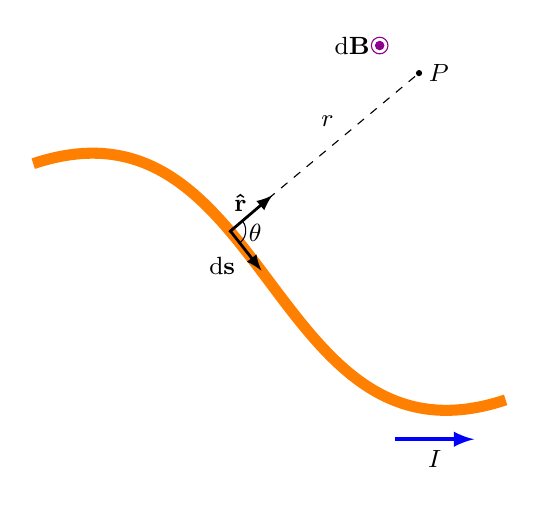
\begin{tikzpicture}[scale=1]
	% Grid
%	\draw[help lines] (0,0) grid (8,8);
	
	% Current Cable	
	\draw[line width=4, color = amber] (1,4) ..controls (4,5) and (4,0).. (7,1) ;
	
	% Vectors
	\draw[dashed] (3.5,3.15)coordinate(B) -- +(2.4,2) node [pos=0.6, above left] {\small$r$};
	\draw[line width = 1,->] (3.5,3.15) -- +(0.4,-0.51)coordinate(A) ;
	\draw[line width = 1,->] (3.49,3.13) -- (4.04,3.6)coordinate(C) node [pos = 0.26, above, black] {\small$\vu{r}$} ;

	
	% Point
	\filldraw (5.9, 5.15) circle (0.9pt) node [right] {\small$P$};
	
	% Nodes
	\node at (3.4,2.7) {\small$\dd\vb{s}$};
	
	% Magnetic Field Direction
	\filldraw[darkmagenta] (5.4, 5.5) circle (1.5pt);
	\filldraw[fill=none, darkmagenta] (5.4, 5.5) circle (3pt) node [left,black] {\small$\dd\vb{B}$};
	
	% Angle
	\pic[draw, angle radius = 0.2cm, angle eccentricity = 1.6, "\small$\theta$"] {angle=A--B--C};
	
	% Current Direction
	\draw[->, blue, line width = 1.5] (5.6,0.5) -- +(1,0) node [midway, below, black] {\small$I$} ;
\end{tikzpicture}
	
\end{document}
